%%%%%%%%%%%%%%%%%%%%%%%%%%%%%%%%%%%%%%%%%%%%%%%%%
%%%%%%%%%%%%%%%%%%%%%%%%%%%%%%%%%%%%%%%%%%%%%%%%%
%%
%%  Modèle pour le  Bulletin de l'Association
%%           mathématique du Québec
%%
%%                 Décembre 2017
%%       Adapté par Marc-André Désautels
%%
%%%%%%%%%%%%%%%%%%%%%%%%%%%%%%%%%%%%%%%%%%%%%%%%%
%%%%%%%%%%%%%%%%%%%%%%%%%%%%%%%%%%%%%%%%%%%%%%%%%


\documentclass[10pt]{article}

%=====================================Ensemble des packages================================

% Ce package sert à accueillir les accents et à faire
% les césures comme on aime qu'elles soient faites en français.
\usepackage[T1]{fontenc}

% Choix de la fonte
\usepackage{lmodern}

%% Permet de traiter les textes accentués
% Pour Windows
\usepackage[utf8]{inputenc}
% Pour Unix
%\usepackage[latin1]{inputenc}
% Pour Apple
%\usepackage[applemac]{inputenc}

% Ensuite, entrer le texte accentué comme à l'ordinaire.
\usepackage[english,french]{babel}

% Permet de rendre le fichier maître plus compatible,
% en particulier avec l'insertion de figures,
% (sauf celle de figures flottantes (package floatingfigure))
% et avec la définition des caractères à doubles jambes.
\usepackage{graphicx}

% Packages qui permettent l'utilisation des symboles et des commandes
% mathématiques de AMS-LaTeX,
\usepackage{amssymb,latexsym,amsmath}

% Package qui donne accès à une police calligraphique, comme eucal.
\usepackage{mathrsfs}

% Package qui permet de fusionner des lignes ou des colonnes de tableaux
\usepackage{multirow}

% Package qui donne accès à la fonte Euler.
\usepackage{euscript}

% Package qui permet de définir ses propres en-têtes et pieds de page.
\usepackage{fancyhdr}

% Package qui permet de passer du texte sur le fichier
% pdf à la ligne du fichier source correspondant.
\usepackage{pdfsync}

% Package permettant de définir son propre style
% de présentation des théorèmes.
\usepackage{theorem}

% Package qui permet au texte de s'enrouler autour de flotants.
\usepackage{wrapfig}
\usepackage{floatflt}

% Package qui "rectifie" les caractères qui dépassent dans la marge.
\usepackage[protrusion=true]{microtype}

% Permet de tracer des graphes flèchés.
% Voir http://www.tug.org/TUGboat/tb22-4/tb72perlax.pdf
\usepackage[all]{xy}

%  Permet de définir les dimensions de la partie imprimée de la page.
% Voir http://ctan.cms.math.ca/tex-archive/macros/latex/contrib/geometry/geometry.pdf
\usepackage{geometry}

% Permet, entre autres, de mettre du texte en filigrane.
% Voir http://math.et.info.free.fr/TikZ/bdd/TikZ-Impatient.pdf
% p. 165
\usepackage{tikz}

% Permet d'utiliser le gabarit de tableaux utilisant les commandes
% of \toprule, \midrule and \bottomrule pour les lignes horizontales dans les tableaux.
\usepackage{booktabs}

\usepackage{color}

% Permet la présentation d'adresses url sous leur forme habituelle.
% Voir http://www.tex.ac.uk/cgi-bin/texfaq2html?label=setURL
\usepackage{url}

% Permet de rendre actifs les liens créés avec le package précédent.
% Voir /usr/local/share/texmf-dist/doc/latex/hyperref/manual.pdf
\usepackage[colorlinks=true,urlcolor=blue, citecolor=cyan, linkcolor=magenta]{hyperref}

% Pour une adresse de courriel: \href{mailto:foo@bar.abc}{Good Link!}
% Pour de belles flèches sur les vecteurs, cadeau de Jean-Philippe Morin
\usepackage{esvect}

%==================================Fin de l'ensemble des packages============================


%=================Pour de belles flèches sur les vecteurs, cadeau de Jean-Philippe Morin=====
\renewcommand{\vec}[1]{\protect\vv{#1}}
% notation de vecteur (\vv définie par package esvect)
% Exemple: \vv{v} ou \vv{AB} ou \vv{A_1A_2}
%============================================================================================


%%%======= Début macro pour numérotation des équations selon les sections du texte==========
%\makeatletter
%\renewcommand\theequation{\thesection.\arabic{equation}}
%\@addtoreset{equation}{section}
%\makeatother
%%%======================  macro: mode d'emploi ============================================
%%% Pour activer cette macro commande, enlever le symbole % au début de la ligne suivante
%\numberwithin{equation}{section}
%%============================================================================================




%%===========Les énoncés ayant la même présentation que les théorèmes=========================
\newtheorem{theorem}{Théorème}
%[section]
\newtheorem{lemma}{Lemme}
%[section]
\newtheorem{proposition}{Proposition}
%[section]
\newtheorem{corollary}{Corollaire}
%[section]
\newtheorem{definition}{Définition}
%[section]
\newtheorem{nota}{Notation}
%[section]
\newtheorem{ex}{Exemple}
%[section]
\newtheorem{nb}{N.B.}
%[section]
\newtheorem{remark}{Remarque}
%%============================================================================================


%%==========================Les démonstrations============================
\newenvironment{proof}
{\par\noindent
\textit{Démonstration}\ }
{
\hfill{$\Box$}
}

%%==============================Les siècles====================================================
%%        Pour la notation des siècles en chiffres romains
%%        La commande est  \siecle{#}
%%        Exemple  \siecle{21}.
%%==========================================================================================
\newcommand{\siecle}[1]{%
\ifnum #1=1%
\uppercase\expandafter{\romannumeral #1}\textsuperscript{er}%
\else%
\uppercase\expandafter{\romannumeral #1}\up{e}%
\fi}

%%=====================================================================
%   Définition des marges pour le Bulletin (NE PAS MODIFIER)
\geometry{height=18.6cm,width=14.4cm}
\geometry{hmargin={3.6cm,3.6cm}}
\geometry{vmargin={4.3cm,5cm}}
%%Ces trois lignes doivent rester avant le \begin{document}.
\parindent=0.0in
\parskip=0.1in
\setcounter{page}{1}
%%=====================================================================

%%========================Caractères particuliers usuels======================
%%
%%==============================Double jambe.============================
\DeclareSymbolFont{AMSb}{U}{msb}{m}{n}
\DeclareSymbolFontAlphabet{\Bbb}{AMSb}
\newcommand{\ds}{\displaystyle}

\usepackage[]{lineno}

\newcommand*\patchAmsMathEnvironmentForLineno[1]{%
  \expandafter\let\csname old#1\expandafter\endcsname\csname #1\endcsname
  \expandafter\let\csname oldend#1\expandafter\endcsname\csname end#1\endcsname
  \renewenvironment{#1}%
     {\linenomath\csname old#1\endcsname}%
     {\csname oldend#1\endcsname\endlinenomath}}%
\newcommand*\patchBothAmsMathEnvironmentsForLineno[1]{%
  \patchAmsMathEnvironmentForLineno{#1}%
  \patchAmsMathEnvironmentForLineno{#1*}}%
\AtBeginDocument{%
\patchBothAmsMathEnvironmentsForLineno{equation}%
\patchBothAmsMathEnvironmentsForLineno{align}%
\patchBothAmsMathEnvironmentsForLineno{flalign}%
\patchBothAmsMathEnvironmentsForLineno{alignat}%
\patchBothAmsMathEnvironmentsForLineno{gather}%
\patchBothAmsMathEnvironmentsForLineno{multline}%
}

%%==========================Packages propres à l'auteur==============================
%%
%% Vous pouvez ajouter ici tous les packages que vous avez besoin.
%% Par exemple

% \usepackage{pstricks}
% \usepackage{enumitem}

%\usepackage{pstricks}
%\usepackage{pst-all}
\usepackage{csquotes}
\usepackage{cancel}
\allowdisplaybreaks

%%
%%==========================Fin des packages propres à l'auteur=======================

%%==========================Commandes propres à l'auteur==============================
%%
%% Vous pouvez ajouter ici toutes les commandes que vous avez définies.
%% Par exemple

% \newcommand{\lr}[1]{\left(#1\right)}
% \newcommand{\abs}[1]{\left\vert#1\right\vert}

\DeclareMathOperator{\Arcsin}{Arcsin}
\DeclareMathOperator{\Arccos}{Arccos}
\DeclareMathOperator{\Arcsec}{Arcsec}
\DeclareMathOperator{\Arccsc}{Arccsc}
\DeclareMathOperator{\Arccot}{Arccot}
\DeclareMathOperator{\Arctan}{Arctan}
\DeclareMathOperator{\Arctanh}{Arctanh}
\DeclareMathOperator{\sech}{sech}
\DeclareMathOperator{\esp}{\mathbb{E}}
\DeclareMathOperator{\var}{Var}
\DeclareMathOperator{\cov}{Cov}
\DeclareMathOperator{\unif}{U}
\newcommand{\lr}[1]{\left(#1\right)}
\newcommand{\abs}[1]{\left\vert#1\right\vert}
\newcommand{\norm}[1]{\left\Vert#1\right\Vert}
\newcommand{\set}[1]{\left\{#1\right\}}
\newcommand{\crochet}[1]{\left[#1\right]}
\newcommand{\comeq}[1]{\quad\lr{\text{#1}}}


%%
%%==========================Fin des commandes propres à l'auteur========================

\usepackage{url}
\usepackage{hyperref}

%%============================pour des barres de fraction obliques=======================
%running fraction with slash - requires math mode.
\newcommand*\rfrac[2]{{}^{#1}\!/_{#2}}
%	Exemple :	\rfrac{3}{7}
%%===============================================================================


%%=== Pour des barres de fraction latérales, une petite, une grande et une très grande ===
\newcommand{\fracinline}[2]{\raisebox{0.4ex}{$#1$} / \raisebox{-0.7ex}{$#2$}}
\newcommand{\bigfracinline}[2]{\raisebox{0.8ex}{$#1$}  \Big/ \raisebox{-1.4ex}{$#2$}}
\newcommand{\biggfracinline}[2]{\raisebox{0.8ex}{$#1$}  \Bigg/ \raisebox{-1.4ex}{$#2$}}

%%	Exemple:	\fracinline{1 + \cos x}{\sin x}
%%	Exemple:	\bigfracinline{1 + \cos x}{\sin x}
%%	Exemple:	\biggfracinline{1 + \cos x}{\sin x}
%%=======================================================================================

\everymath{\displaystyle}


\begin{document}

%%==========================Éléments propres à l'auteur==============================
%%
%%
%%==========================Fin des éléments propres à l'auteur======================


%%=====================Pour mettre le titre des tableaux en français==================
%%
\renewcommand{\tablename}{\textsc{Tableau}}
%%
%%=========================Fin de la nouvelle définition==============================

\begin{center}
\textsf{\LARGE \textbf{Le problème du char d'assaut allemand}}
\end{center}

\begin{flushright}
\textsc{Marc-André Désautels, département de mathématiques} \\
\textsc{Cégep de Saint-Jean-sur-Richelieu} \\
\href{mailto:marc-andre.desautels@cstjean.qc.ca}{marc-andre.desautels@cstjean.qc.ca} \\
\href{https://www.cstjean.qc.ca/}{https://www.cstjean.qc.ca/}
\end{flushright}


\baselineskip=1.2\baselineskip

%%=====================================================================
%%          Résumé
%%=====================================================================

\begin{abstract}

Durant la seconde guerre mondiale, les alliés avaient un besoin criant
d'estimer avec précision la quantité de matériel militaire que
l'Allemagne nazie produisait. Les estimations provenant des services de
renseignements habituels étaient contradictoires et incertaines. Les
gouvernements Britanniques et Américains se tournèrent donc vers des
statisticiens pour savoir si leurs estimations pouvaient être
améliorées. Nous présenterons une introduction aux notions mathématiques
utilisées.

\end{abstract}
%%=====================================================================
%%          Fin du résumé
%%=====================================================================

\textbf{Mots clés: } Statistiques, Estimation, Simulation

\bigskip

\hypertarget{introduction}{%
\section{\texorpdfstring{Introduction
\label{intro}}{Introduction }}\label{introduction}}

Au début de l'année 1943, la \emph{Economic Warfare Division} de
l'ambassade américaine à Londres commença à analyser divers marquages
obtenus à partir d'équipements allemands capturés ou détruits sur le
front. Plus particulièrement, les numéros de séries ont été utilisés
pour estimer la force de production de la machine de guerre allemande.
L'article \emph{An Empirical Approach to Economic Intelligence in World
War II} \cite{Ruggles1947} explique en grand détail le développement des
techniques utilisés pour faire cette estimation, les problèmes
rencontrés et les solutions qui y ont remédiés. Nous invitons le lecteur
intéressé par l'aspect pratico-pratique de ces techniques à lire cet
article.

Le problème du char d'assaut allemand est nommé d'après son application
par les alliés à l'estimation du nombre de chars d'assaut produits par
l'Allemagne. Mais en fait, ce problème regroupe l'estimation du nombre
de nombreux produits de guerre allemands, par exemple les camions, les
fusils, les bombes et les fusées, voir \cite{Ruggles1947}. En
particulier, nous présentons au tableau \ref{tab:estimation_ruggles} les
estimations du nombre de chars d'assaut allemands en comparaison avec
l'estimation par les services de renseignements et les archives
allemandes, tel que présenté dans \cite{Ruggles1947}.

\begin{table}[ht]
\begin{center}
\begin{tabular}{cccc}
\multirow{2}{*}{Mois} & \multirow{2}{*}{Estimation statistique} & Estimation par les & Selon les archives \\
& & services de renseignements &  allemandes \\
\hline
\hline
Juin 1940 & 169 & 1 000 & 122 \\
Juin 1941 & 244 & 1 550 & 271 \\
Août 1942 & 327 & 1 550 & 342 \\
\hline
\end{tabular}
\end{center}
\caption{\label{tab:estimation_ruggles} {Comparaison des estimations produites par les estimateurs que nous présenterons, des estimations produites par les services de renseignements ainsi que de la production exacte selon les archives allemandes.} }
\end{table}

Les russes ont également utilisé des techniques similaires pour estimer
la production de char d'assaut allemands \cite{Volz2008}. Durant les
années 80, des militaires Américains ont eu accès aux lignes de
production de chars d'assaut \emph{Merkava} israéliens. Le nombre de
chars produits était confidentiel, mais le colone Dupuy indique que
puisque chaque chars possédait un numéro de série, il aurait pu estimer
la production, voir \cite{Johnson}

Les formules développées dans cet article ont aussi été utilisées dans
des contextes non-militaires. Par exemple, elles ont été utilisées pour
estimer le nombre de \emph{Commodore 64} produits, voir
\cite{commodore64}. Le premier modèle de iPhone, commercialisé en 2007
aux États-Unis, a été vendu au nombre de 9 190 680, suite à des
estimations faites à partir des codes IMEI (\emph{The International
Mobile Equipment Identity}) de nombreux utilisateurs, voir
\cite{iphone}.

Dans cet article, nous nous intéresserons à l'estimation du nombre
d'items \(N\) à partir d'un échantillon aléatoire dans le cas où les
items sont numérotés de façon séquentielle.

\hypertarget{les-mathematiques}{%
\section{\texorpdfstring{Les mathématiques
\label{maths}}{Les mathématiques }}\label{les-mathematiques}}

\hypertarget{prealables}{%
\subsection{Préalables}\label{prealables}}

Supposons que nous avons une population d'objets numérotés de la façon
suivante : \(1\), \(2\), \(3\), \ldots{} , \(N\), où \(N\) est
\textbf{inconnu}. En d'autres mots, les objets de notre population
doivent être numérotés de façon \emph{séquentielle}. Nous pigeons,
\textbf{sans remise}, un échantillon \(X_1\), \(X_2\), \(X_3\),
\ldots{}, \(X_n\), de taille \(n\) à partir de la population. Nous
voulons estimer la valeur de \(N\) à partir de l'échantillon prélevé.

Pour calculer les diverses mesures statistiques dont nous aurons besoin,
nous allons classer les unités statistiques de notre échantillon en
ordre croissant. Nous avons:
\[X_{(1)} <  X_{(2)} < X_{(3)} < \ldots < X_{(n-1)} < X_{(n)}\] où les
valeurs \(X_{(1)}\), \(X_{(2)}\), \(X_{(3)}\), \ldots{}, \(X_{(n)}\)
sont les valeurs ordonnées de l'échantillon \(X_1\), \(X_2\), \(X_3\),
\ldots{}, \(X_n\). En particulier, \(X_{(1)}\) est la plus petite valeur
de l'échantillon et \(X_{(n)}\) est la plus grande.

À partir de nos définitions précédentes, il est possible de calculer
l'espérance de la valeur \(X_{(A)}\) (\(\esp (X_{(A)})\)), la variance
de la valeur \(X_{(A)}\) (\(\var(X_{(A)})\)) et enfin la covariance des
valeurs \(X_{(A)}\) et \(X_{(B)}\) (\(\cov(X_{(A)},X_{(B)})\)). Nous
utiliserons ces mesures statistiques pour calculer l'espérance et la
variance des estimateurs que nous construirons. Malheureusement,
retrouver ces mesures statistiques nécessite des identités combinatoires
et de fastidieux calculs. Pour ne pas alourdir le texte, nous donnerons
ces mesures sans démonstration. Par contre, pour la lectrice ou le
lecteur intéressé, vous pourrez trouver à l'annexe \ref{calculs_proba}
une idée de la technique utilisée ainsi que la démonstration de
\(\esp(X_{(A)})\).

Nous utiliserons donc, sans démonstration, les trois mesures du tableau
\ref{tab:mesures_stat}. La lectrice ou le lecteur curieux pourront aller
aux annexes \ref{rappel_esperance} et \ref{calculs_proba} pour quelques
rappels sur les notions d'espérance, de variance et de covariance ainsi
que la démonstration de \(\esp(X_{(A)})\). Les démonstrations de
\(\var(X_{(A)})\) et \(\cov(X_{(A)},X_{(B)})\) se font d'une manière
similaire.

\begin{table}[ht]
\begin{center}
\begin{tabular}{|r|c|}
\hline
Mesure & Formule \\
\hline
\hline
$\esp (X_{(A)})$ & $\frac{A(N+1)}{n+1}$ \\ 
\hline
$\var(X_{(A)})$ & $\frac{A(n+1-A)(N+1)(N-n)}{(n+1)^2(n+2)}$ \\
\hline
$\cov(X_{(A)},X_{(B)})$ & $\frac{A(n+1-B)(N+1)(N-n)}{(n+1)^2(n+2)}$ \\
\hline
\end{tabular}
\end{center}
\caption{\label{tab:mesures_stat} {Les mesures de l'espérance, de la variance et de la covariance pour une valeur $X_{(A)}$ de notre échantillon.} }
\end{table}

À l'aide des trois mesures du tableau \ref{tab:mesures_stat}, nous
allons maintenant trouver quatre estimés de \(N\) en utilisant
simplement notre ``gros bon sens''. La structure des prochaines sections
est calquée sur \cite{Johnson}. Nous utiliserons aussi les notions
présentées en \cite{Goodman1952} et \cite{Goodman1954}.

\hypertarget{les-trois-situations-possibles}{%
\subsection{Les trois situations
possibles}\label{les-trois-situations-possibles}}

Supposons que nous avons une population d'objets numérotés de la façon
suivante : \(s+1\), \(s+2\), \(s+3\), \ldots{} , \(s+N\). Trois
situations distinctes peuvent se produire:

\begin{enumerate}
\def\labelenumi{\arabic{enumi}.}
\item
  \(s\) est \textbf{connu} et égal à \(0\) et \(N\) est
  \textbf{inconnu}.
\item
  \(s\) est \textbf{connu} mais différent de \(0\) et \(N\) est
  \textbf{inconnu}.
\item
  \(s\) est \textbf{inconnu} et \(N\) est \textbf{inconnu}.
\end{enumerate}

Nous étudierons, dans l'ordre, les trois situations précédentes.

\hypertarget{la-situation-ou-s-est-connu-et-egal-a-0-et-n-est-inconnu}{%
\subsection{\texorpdfstring{La situation où \(s\) est \textbf{connu} et
égal à \(0\) et \(N\) est
\textbf{inconnu}}{La situation où s est connu et égal à 0 et N est inconnu}}\label{la-situation-ou-s-est-connu-et-egal-a-0-et-n-est-inconnu}}

Puisque \(s\) est connu et égal à \(0\), nous nous trouvons dans la
situation où notre liste est numérotée de la façon suivante : \(1\),
\(2\), \ldots{}, \(N\). Cette situation est en fait un cas particulier
d'une loi uniforme discrète de la forme \(\unif(1,N)\).

\hypertarget{le-milieu-de-la-liste}{%
\subsubsection{Le milieu de la liste}\label{le-milieu-de-la-liste}}

Pour trouver nos deux premiers estimateurs, nous allons débuter en
supposant que nous connaissons la valeur milieu \(m\) de la liste \(1\),
\(2\), \ldots{}, \(N\). Nous nous retrouvons dans la situation
ci-dessous:
\[\underbrace{1,2,3,\ldots,m-1}_{m-1 \text{ éléments}},m,\underbrace{m+1,\ldots,N-2,N-1,N}_{m-1 \text{ éléments}}\]
Il y aura donc \(m-1\) valeurs en-dessous de \(m\) et \(m-1\) valeurs
au-dessus de \(m\). Donc, si nous incluons la valeur milieu \(m\), nous
avons \(N=(m-1)+1+(m-1)=2m-1\). Puisque nous ne connaissons pas la
valeur milieu \(m\), il est raisonnable de la remplacer par une
estimation, par exemple la médiane \(\widetilde{X}\) ou la moyenne
\(\overline{X}\). Nous pouvons maintenant obtenir nos deux premiers
estimateurs.

\begin{quote}
À partir de maintenant, nous allons toujours supposer que nous
arrondissons nos estimateurs à l'entier le plus près.
\end{quote}

\hypertarget{la-mediane}{%
\subsubsection{La médiane}\label{la-mediane}}

Nous noterons notre premier estimateur
\(\widehat{N_1}=2\widetilde{X}-1\), où \(\widetilde{X}\) représente la
médiane de notre échantillon. Rappelons que pour \(k\) données
discrètes, la médiane se calcule de deux façons différentes,
dépendamment du fait que le nombre de données soit pair ou impair.
\begin{align*}
\widetilde{X} &= 
\begin{cases}
\frac{1}{2}\lr{X_{\lr{k/2}}+X_{\lr{k/2+1}}} & \text{ si $k$ est pair} \\
X_{\lr{(k+1)/2}} & \text{ si $k$ est impair} \\
\end{cases}
\end{align*} Nous voulons vérifier si l'estimateur \(\widehat{N_1}\) est
non-biaisé, c'est-à-dire si l'espérance de \(\widehat{N_1}\) est égale à
\(N\) (\(\esp (\widehat{N_1})=N\)). Nous voulons également calculer la
variance de \(\widehat{N_1}\). Pour éviter d'alourdir le texte, nous
avons mis un exemple de calcul d'espérance et de variance à l'annexe
\ref{calculs_estimateurs}. En effectuant les calculs appropriés, nous
obtenons les résultats du tableau \ref{tab:estimateur_n1}.

\begin{table}[ht]
\begin{center}
\begin{tabular}{|c|c|c|c|}
\hline
$i$ & $\widehat{N_i}$ & $\esp\lr{\widehat{N_i}}$ & $\var\lr{\widehat{N_i}}$ \\
\hline
\hline
\multirow{2}{*}{1}  & \multirow{2}{*}{$2\widetilde{X}-1$} & \multirow{2}{*}{$N$} & 
$\frac{(N-n)(N+1)}{n+2}$ pour $n$ impair \\
& & & $\frac{n}{n+1}\frac{(N-n)(N+1)}{n+2}$ pour $n$ pair \\
\hline
\end{tabular}
\end{center}
\caption{\label{tab:estimateur_n1} {L'espérance et la variance de l'estimateur $\widehat{N_1}$.} }
\end{table}

\hypertarget{la-moyenne}{%
\subsubsection{La moyenne}\label{la-moyenne}}

Notre second estimateur est \(\widehat{N_2}=2\overline{X}-1\), où
\(\overline{X}\) représente la moyenne de notre échantillon. Rappelons
que pour \(k\) données discrètes, la moyenne se calcule de la façon
suivante: \begin{align*}
\overline{X} &= \dfrac{X_{(1)}+X_{(2)}+\ldots +X_{(k-1)}+X_{(k)}}{k}
\end{align*} En effectuant les calculs appropriés pour l'espérance et la
variance, nous obtenons les résultats du tableau
\ref{tab:estimateur_n2}.

\begin{table}[ht]
\begin{center}
\begin{tabular}{|c|c|c|c|}
\hline
$i$ & $\widehat{N_i}$ & $\esp\lr{\widehat{N_i}}$ & $\var\lr{\widehat{N_i}}$ \\
\hline
\hline
2 & $2\overline{X}-1$ & $N$ & $\frac{n+2}{3n}\frac{(N-n)(N+1)}{n+2}$ \\
\hline
\end{tabular}
\end{center}
\caption{\label{tab:estimateur_n2} {L'espérance et la variance de l'estimateur $\widehat{N_2}$.} }
\end{table}

Malheureusement, nos deux estimés \(\widehat{N_1}\) et \(\widehat{N_2}\)
présentent un problème. Les valeurs de ces deux estimateurs peuvent être
plus petites que le plus grand entier dans notre échantillon,
c'est-à-dire \(X_{(n)}\). Il est bien sûr impossible que la valeur \(N\)
que nous cherchons soit plus petite que la plus grande valeur de notre
échantillon.

Pour vous convaincre, étudions l'échantillon de taille \(n=5\) suivant,
tel que \(X_1=2\), \(X_2=10\), \(X_3=3\), \(X_4=1\) et \(X_5=4\). Dans
cette situation, la médiane de l'échantillon est 3 et la moyenne est 5.
Nous obtenons donc:
\[\widehat{N_1}=2\widetilde{X}-1=5 \qquad \text{et} \qquad \widehat{N_2}=2\overline{X}-1=9 \]
Malheureusement, nous savons que \(N\) est supérieur ou égal à 10, le
maximum de notre échantillon. Ces deux estimateurs ne sont donc pas
adéquats, nous devrons en trouver d'autres.

\hypertarget{deux-autres-estimes}{%
\subsubsection{Deux autres estimés}\label{deux-autres-estimes}}

Nous voulons maintenant trouver d'autres estimés qui sont toujours
supérieurs ou égaux au plus grand entier de notre échantillon. Par
symétrie, nous pouvons supposer que le nombre de numéros de série
non-observés au-dessus de \(X_{(n)}\) soit le même que le nombre de
numéros de série non-observés en-dessous de \(X_{(1)}\). Nous avons
donc: \begin{align*}
N-X_{(n)} &= X_{(1)}-1 \\
\widehat{N_3} &= X_{(n)}+X_{(1)}-1
\end{align*} En effectuant les calculs appropriés pour l'espérance et la
variance, nous obtenons les résultats du tableau
\ref{tab:estimateur_n3}.

\begin{table}[ht]
\begin{center}
\begin{tabular}{|c|c|c|c|}
\hline
$i$ & $\widehat{N_i}$ & $\esp\lr{\widehat{N_i}}$ & $\var\lr{\widehat{N_i}}$ \\
\hline
\hline
3 & $X_{(n)}+X_{(1)}-1$ & $N$ & $\frac{2}{n+1}\frac{(N-n)(N+1)}{n+2}$ \\
\hline
\end{tabular}
\end{center}
\caption{\label{tab:estimateur_n3} {L'espérance et la variance de l'estimateur $\widehat{N_3}$.} }
\end{table}

Nous pouvons continuer le raisonnement précédent. En effet, il apparaît
raisonnable de poser le nombre de numéros de série non-observés
au-dessus de \(X_{(n)}\) comme étant la moyenne du:

\begin{itemize}
\item
  nombre de numéros de série non-observés en-dessous de \(X_{(1)}\);
\item
  nombre de numéros de série non-observés entre \(X_{(1)}\) et
  \(X_{(2)}\);
\item
  nombre de numéros de série non-observés entre \(X_{(2)}\) et
  \(X_{(3)}\);
\item
  \ldots{}
\item
  nombre de numéros de série non-observés entre \(X_{(n-1)}\) et
  \(X_{(n)}\).
\end{itemize}

Nous avons donc que le nombre de numéros de série non-observés au-dessus
de \(X_{(n)}\), c'est-à-dire \(N-X_{(n)}\) est égal à: \begin{align*}
N-X_{(n)} &= \frac{1}{n}\left[ (X_{(1)}-1)+(X_{(2)}-X_{(1)}-1)+(X_{(3)}-X_{(2)}-1)+\ldots+(X_{(n)}-X_{(n-1)}-1) \right] \\
&= \frac{X_{(n)}}{n}-1 \\
\widehat{N_4} &= \lr{\frac{n+1}{n}} X_{(n)}-1
\end{align*} En effectuant les calculs appropriés pour l'espérance et la
variance, nous obtenons les résultats du tableau
\ref{tab:estimateur_n4}.

\begin{table}[ht]
\begin{center}
\begin{tabular}{|c|c|c|c|}
\hline
$i$ & $\widehat{N_i}$ & $\esp\lr{\widehat{N_i}}$ & $\var\lr{\widehat{N_i}}$ \\
\hline
\hline
4 & $\lr{\frac{n+1}{n}} X_{(n)}-1$ & $N$ & $\frac{1}{n}\frac{(N-n)(N+1)}{n+2}$ \\
\hline
\end{tabular}
\end{center}
\caption{\label{tab:estimateur_n4} {L'espérance et la variance de l'estimateur $\widehat{N_4}$.} }
\end{table}

Bien que la démonstration des résultats présentés aux tableaux
\ref{tab:estimateur_n1}, \ref{tab:estimateur_n2},
\ref{tab:estimateur_n3} et \ref{tab:estimateur_n4} ne soit pas
présentée, nous pouvons remarquer les résultats suivants:

\begin{itemize}
\item
  Dans le cas où \(n=1\), la variance des quatre estimateurs est la
  même.
\item
  Dans le cas où la taille de notre échantillon est la même que celle de
  notre population, c'est-à-dire \(n=N\), les variances de nos quatre
  estimateurs sont nulles.
\item
  Les variances de nos estimateurs diminuent lorsque \(i\) augmente, ce
  qui indique que \(\widehat{N_4}\) est l'estimateur ayant la variance
  la plus petite.
\item
  Il est possible d'utiliser le théorème de Lehmann-Scheffé pour
  démontrer que \(\widehat{N_4}\) est l'estimateur non-biaisé ayant la
  plus petite variance.
\end{itemize}

La lectrice ou le lecteur intéressé pourront utiliser les idées
présentées à l'annexe \ref{calculs_estimateurs} pour démontrer les
résultats des tableaux \ref{tab:estimateur_n1}, \ref{tab:estimateur_n2},
\ref{tab:estimateur_n3} et \ref{tab:estimateur_n4}.

\hypertarget{la-situation-ou-s-est-connu-mais-different-de-0-et-n-est-inconnu}{%
\subsection{\texorpdfstring{La situation où \(s\) est \textbf{connu}
mais différent de \(0\) et \(N\) est
\textbf{inconnu}}{La situation où s est connu mais différent de 0 et N est inconnu}}\label{la-situation-ou-s-est-connu-mais-different-de-0-et-n-est-inconnu}}

Supposons que nous avons une population d'objets numérotés de la façon
suivante : \(s+1\), \(s+2\), \(s+3\), \ldots{} , \(s+N\), où \(N\) est
inconnu mais \(s\) est \textbf{connu}. Cette situation est en fait un
cas particulier d'une loi uniforme discrète de la forme
\(\unif(s+1,s+N)\).

Nous pouvons résoudre ce problème en utilisant les estimés précédents et
en soustrayant la valeur \(s\) aux numéros de série obtenus.

\hypertarget{la-situation-ou-s-est-inconnu-et-n-est-inconnu}{%
\subsection{\texorpdfstring{La situation où \(s\) est \textbf{inconnu}
et \(N\) est
\textbf{inconnu}}{La situation où s est inconnu et N est inconnu}}\label{la-situation-ou-s-est-inconnu-et-n-est-inconnu}}

Supposons que nous avons une population d'objets numérotés de la façon
suivante : \(s+1\), \(s+2\), \(s+3\), \ldots{} , \(s+N\), où \(N\) est
inconnu mais \(s\) est lui aussi \textbf{inconnu}. Cette situation était
celle des numéros de séries sur les boîtes de transmissions des chars
d'assaut \emph{Panther V}, comme présenté en \cite{Ruggles1947}. Nous
avons trouvé à l'annexe \ref{calculs_proba} les espérances des valeurs
\(X_{(A)}\) de notre échantillon, c'est-à-dire
\(\esp (X_{(A)})=\frac{A(N+1)}{n+1}\).

Nous allons étudier l'espérance de la différence \(d\) entre le plus
grand \((X_{(n)})\) et le plus petit \((X_{(1)})\) des numéros de série
de notre échantillon. Ce résultat reste vrai même dans la situation où
\(s\) est inconnu. Nous avons donc: \begin{align*}
\esp(X_{(n)}-X_{(1)}) &= \esp(X_{(n)})-\esp(X_{(1)}) \\
X_{(n)}-X_{(1)} &= \dfrac{n\cdot(N+1)}{n+1}-\dfrac{1\cdot(N+1)}{n+1} \\
&= \dfrac{(n-1)(N+1)}{n+1} \\
N+1 &= \dfrac{(X_{(n)}-X_{(1)})(n+1)}{n-1} \\
\widehat{N_5} &= \dfrac{(X_{(n)}-X_{(1)})(n+1)}{n-1}-1
\end{align*} Il est donc possible d'estimer la taille de la population,
même si \(s\) et \(N\) sont inconnus. En effectuant les calculs
appropriés pour l'espérance et la variance, nous obtenons les résultats
du tableau \ref{tab:estimateur_n5}.

\begin{table}[ht]
\begin{center}
\begin{tabular}{|c|c|c|c|}
\hline
$i$ & $\widehat{N_i}$ & $\esp\lr{\widehat{N_i}}$ & $\var\lr{\widehat{N_i}}$ \\
\hline
\hline
5 & $\dfrac{(X_{(n)}-X_{(1)})(n+1)}{n-1}-1$ & $N$ & $\frac{2}{n-1}\frac{(N-n)(N+1)}{n+2}$ \\
\hline
\end{tabular}
\end{center}
\caption{\label{tab:estimateur_n5} {L'espérance et la variance de l'estimateur $\widehat{N_5}$.} }
\end{table}

\hypertarget{quelques-simulations}{%
\section{\texorpdfstring{Quelques simulations
\label{simul}}{Quelques simulations }}\label{quelques-simulations}}

Pour visualiser les différences entre les cinq estimateurs trouvés, nous
allons effectuer des simulations avec le logiciel \texttt{R}. Les
commandes \texttt{R} utilisées seront précédées du symbole
\texttt{\textgreater{}}, qui représente l'invite de commandes
(\emph{prompt} en anglais). Ce symbole indique que l'interface de
\texttt{R} est prête à recevoir une commande.

Pour nos simulations, nous utiliserons une population de taille
\(N=500\). Nous pouvons créer cette population dans \texttt{R} de la
façon suivante:

\begin{verbatim}
> pop <- c(1:500)
\end{verbatim}

Pour modéliser le problème qui nous intéresse, nous voulons piger, sans
remise (d'où l'ajout de l'option \texttt{replace=FALSE}), un échantillon
de notre population. Pour cette première simulation, nous pigerons un
échantillon de taille \(n=5\).

\begin{verbatim}
> ech <- sample(pop, 5, replace = FALSE)
> ech
\end{verbatim}

\begin{verbatim}
## [1] 349  23 152  28 105
\end{verbatim}

Le minimum de notre échantillon est 23 et le maximum est 349. Nous
pouvons calculer les cinq estimateurs associés à l'échantillon
précédent:

\begin{verbatim}
> N1(ech)
## [1] 209
> N2(ech)
## [1] 262
> N3(ech)
## [1] 371
> N4(ech)
## [1] 418
> N5(ech)
## [1] 488
\end{verbatim}

À partir d'ici, pour ne pas alourdir le texte, nous omettrons le code
\texttt{R} utilisé pour produire les simulations qui suivent. Vous
trouverez par contre à l'annexe \ref{code} le code complet utilisé.

Pour bien visualiser les différences entre nos cinq estimateurs, nous
effectuerons quatre simulations distinctes. La figure \ref{fig:fig-ech}
représente une simulation de 5 000 échantillons de tailles 5, 10, 25 et
50, à partir d'une population de taille 500. Nous calculons les mesures
de nos cinq estimateurs pour ces 5 000 échantillons.

\begin{figure}[!htb]

{\centering 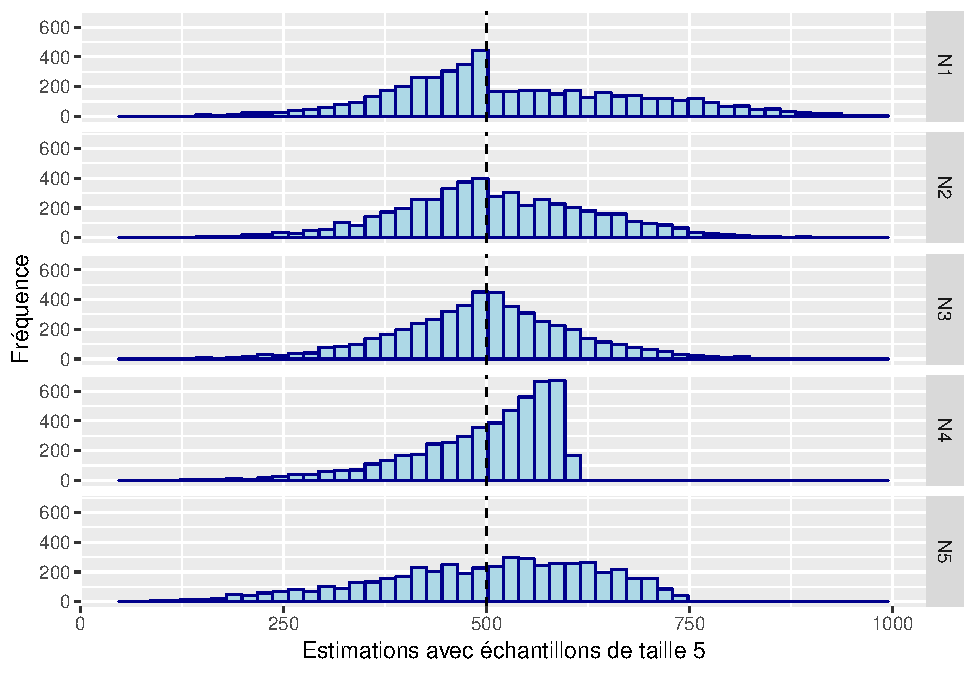
\includegraphics[width=0.48\linewidth]{serial_number_amq_files/figure-latex/fig-ech-1} 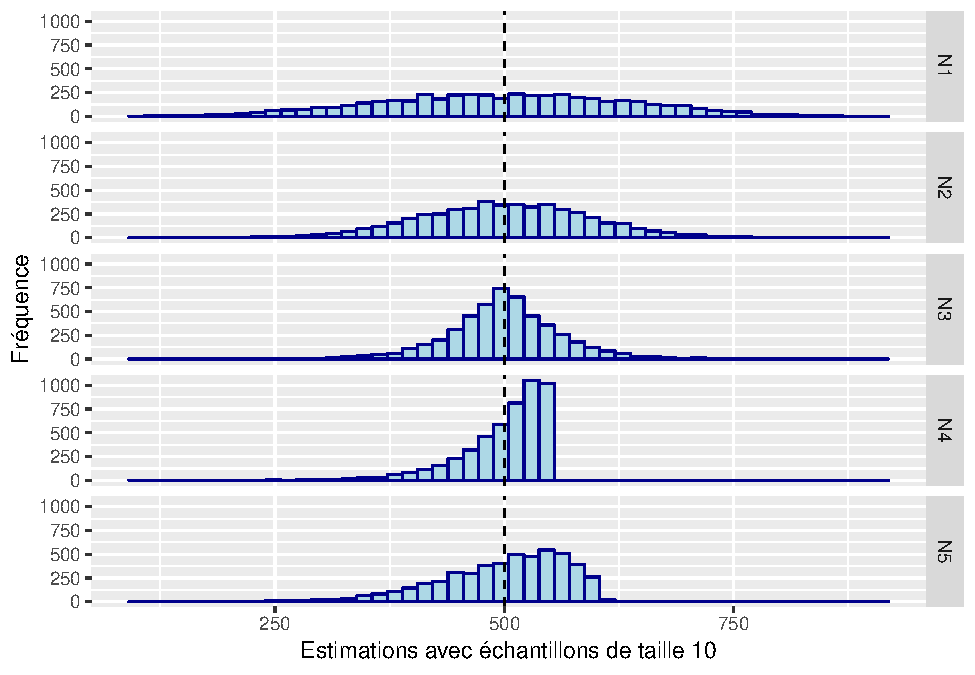
\includegraphics[width=0.48\linewidth]{serial_number_amq_files/figure-latex/fig-ech-2} 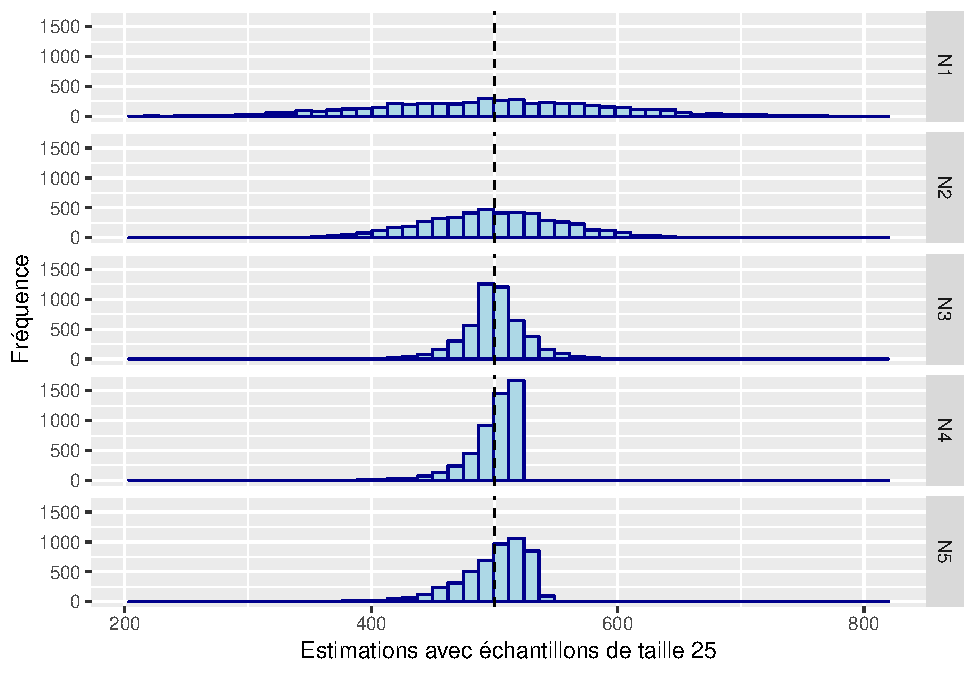
\includegraphics[width=0.48\linewidth]{serial_number_amq_files/figure-latex/fig-ech-3} 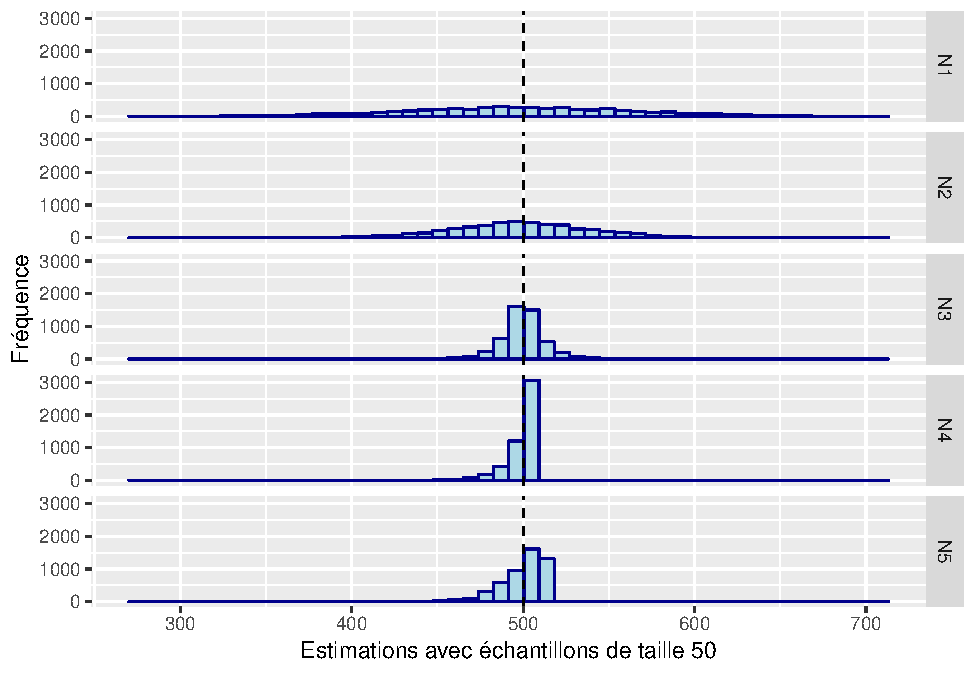
\includegraphics[width=0.48\linewidth]{serial_number_amq_files/figure-latex/fig-ech-4} 

}

\caption{Représentation sous forme d'histogrammes de 5 000 échantillons de taille 5 (en haut à gauche), de taille 10 (en haut à droite), de taille 25 (en bas à gauche) et de taille 50 (en bas à droite) pour les cinq estimateurs. La ligne pointillée correspond à la taille de la population, c'est-à-dire 500.}\label{fig:fig-ech}
\end{figure}

Pour représenter différemment les résultats de nos cinq estimateurs,
nous ferons un autre type de simulation. Nous allons faire varier la
taille de la population de 10 à 1000, par bonds de 5. Pour chacunes de
ces populations, nous choisissons un échantillon de taille 5 et nous
calculons la valeur des cinq estimateurs. Pour être en mesure de bien
visualiser les résultats, nous allons ajouter une petite variation
aléatoire à la position des points. De cette façon, nous verrons mieux
la dispersion de nos données. La figure \ref{fig:ech-10-1000} représente
nos résultats obtenus à partir de nos échantillons pour les cinq
estimateurs. La droite en rouge représente la taille véritable de la
population. Les idées utilisées pour obtenir les graphiques de la figure
\ref{fig:ech-10-1000} sont basées sur \cite{Hinno}.

\begin{figure}[!htb]

{\centering 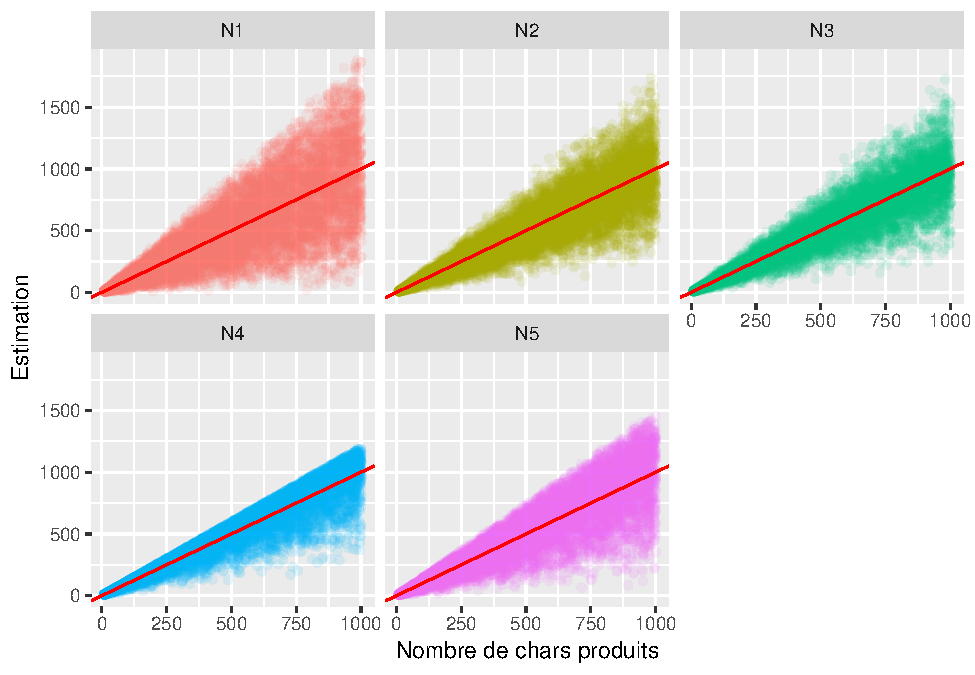
\includegraphics[width=0.9\linewidth]{serial_number_amq_files/figure-latex/ech-10-1000-1} 

}

\caption{Représentation de 50 échantillons de taille 5 pigés pour des populations de tailles 10 à 1 000, pour les cinq estimateurs. La droite en rouge représente la taille véritable de la population.}\label{fig:ech-10-1000}
\end{figure}

Nous allons maintenant partir d'une population de taille 500. Nous
ferons varier la taille des échantillons de 1 à 500, par bonds de 1.
Pour chacune de ces tailles, nous pigerons 50 échantillons sans remise.
Nous représenterons ensuite l'estimation obtenu en fonction de la taille
des échantillons. Pour être en mesure de bien visualiser les résultats,
nous allons ajouter une petite variation aléatoire à la position des
points. La figure \ref{fig:pop-1-500} représente nos résultats obtenus.

\begin{figure}[!htb]

{\centering 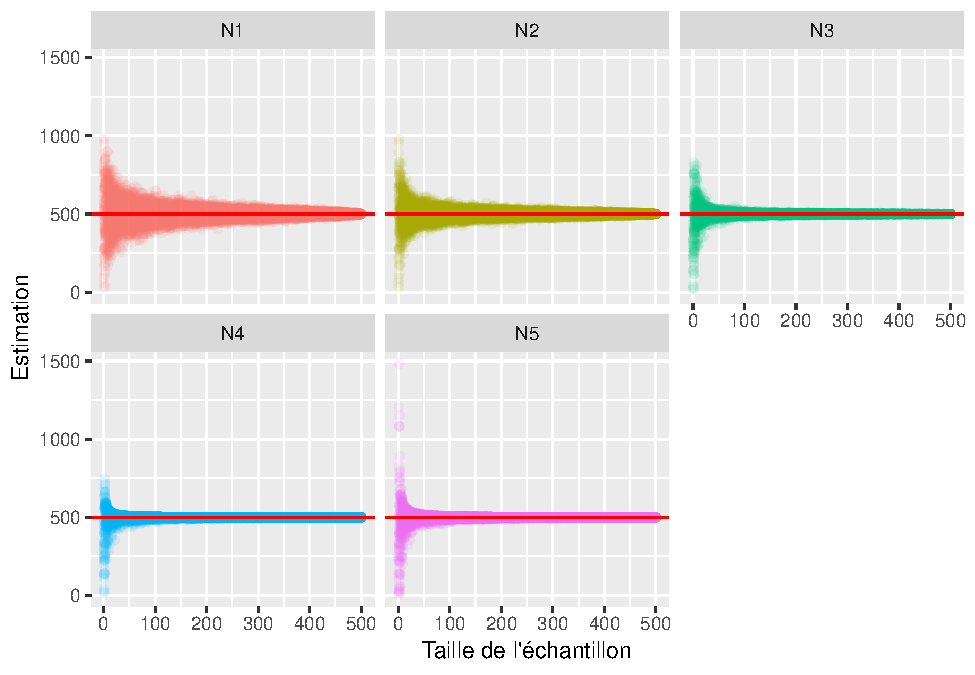
\includegraphics[width=0.9\linewidth]{serial_number_amq_files/figure-latex/pop-1-500-1} 

}

\caption{Représentation de 50 échantillons de taille 1 à 500 pigés pour une population de taille 500, pour les cinq estimateurs. La droite en rouge représente la taille véritable de la population.}\label{fig:pop-1-500}
\end{figure}

\hypertarget{une-application}{%
\section{\texorpdfstring{Une application
\label{application}}{Une application }}\label{une-application}}

Nous trouvons en \cite{Goodman1954} une application concrète de
l'utilisation de nos estimateurs. On nous indique que le département des
sciences sociales de l'Université de Chicago utilisaient de l'équipement
(bureaux, chaises, etc.) sur lesquels étaient placés des numéros de
série.

Les numéros de série de 31 pièces d'équipement ont été observées. Les 31
numéros de série étaient:

\begin{verbatim}
##  [1]   83  135  274  380  668  895  955  964 1113 1174 1210 1344 1387 1414
## [15] 1610 1668 1689 1756 1865 1874 1880 1936 2005 2006 2065 2157 2220 2224
## [29] 2396 2543 2787
\end{verbatim}

Nous invitons les lectrices et les lecteurs intéressés à utiliser les
cinq estimateurs présentés dans cet article pour estimer le nombre
d'équipements achetés par l'Université de Chicago. Le minimum de
l'échantillon est 83 et le maximum de l'échantillon est 2787. Les
réponses des cinq estimateurs ainsi que la véritable valeur du nombre
d'équipements seront donnés à l'annexe \ref{rep-application}.

\appendix

\hypertarget{rappels}{%
\section{\texorpdfstring{Rappels
\label{rappel_esperance}}{Rappels }}\label{rappels}}

\begin{definition}[Espérance d'une variable discrète prenant un nombre fini de valeurs]
Soit $X$ une variable aléatoire discrète avec un nombre fini de valeurs $x_1$, $x_2$, ..., $x_k$ auxquelles sont associées les probabilités $p_1$, $p_2$, ..., $p_k$. L'espérance de $X$, notée $\esp (X)$ est définie comme:
$$ \esp (X) = x_1p_1+x_2p_2+\ldots +x_kp_k = \sum_{i=1}^k x_i p_i $$
\end{definition}

Voici quelques propriétés élémentaires concernant l'espérance de
variables aléatoires.

\begin{itemize}
\item
  Soit \(k\in\mathbb{R}\), alors \(\esp(k)=k\).
\item
  Soit \(X_i\) où \(i\in\set{1,2,\ldots,n}\), \(n\) variables aléatoires
  définies sur le même espace probabiliste et \(a_i\in\mathbb{R}\),
  alors \(\esp\lr{\sum_{i=1}^na_iX_i}=\sum_{i=1}^n a_i\esp(X_i)\).
\end{itemize}

\begin{definition}[Variance]
Soit $X$ une variable aléatoire discrète avec un nombre fini de valeurs $x_1$, $x_2$, ..., $x_k$ auxquelles sont associées les probabilités $p_1$, $p_2$, ..., $p_k$. La variance de $X$, notée $\var (X)$ est définie comme:
$$ \var (X) = \esp\crochet{\lr{X-\esp(X)}^2} $$
\end{definition}

\begin{definition}[Covariance]
Soit $X$ et $Y$ deux variables aléatoires définies sur le même espace probabiliste et ayant chacune une variance finie. La covariance de $X$ et $Y$, notée $\cov(X,Y)$ est définie comme:
$$ \cov(X,Y)=\esp\crochet{\lr{X-\esp(X)}\lr{Y-\esp(Y)}} $$
\end{definition}

Voici quelques propriétés élémentaires concernant la variance et la
covariance de variables aléatoires.

\begin{itemize}
\item
  Le théorème de König-Huygens donne la formule de variance alternative
  suivante: \(\var(X)=\esp(X^2)-\lr{\esp(X)}^2\).
\item
  Soit \(X\) une variable aléatoire et \(a,b\in\mathbb{R}\), alors
  \(\var(aX+b)=a^2\var(X)\).
\item
  Soit \(X_i\) où \(i\in\set{1,2,\ldots,n}\), \(n\) variables aléatoires
  définies sur le même espace probabiliste et \(a_i\in\mathbb{R}\),
  alors
  \(\var\lr{\sum_{i=1}^n a_iX_i}=\sum_{i=1}^n a_i^2\var(X_i)+2\sum_{1\leq i< j\leq n} a_ia_j\cov(X_i,X_j)\).
\item
  Une généralisation du théorème de König-Huygens pour la variance
  implique: \(\cov(X,Y)=\esp(XY)-\esp(X)\esp(Y)\).
\item
  \(\cov(X,X)=\var(X)\)
\item
  \(\cov(X,Y)=\cov(Y,X)\)
\end{itemize}

\hypertarget{calcul-de-probabilites}{%
\section{\texorpdfstring{Calcul de probabilités
\label{calculs_proba}}{Calcul de probabilités }}\label{calcul-de-probabilites}}

Nous voulons calculer la probabilité reliée à l'événement \(X_{(A)}=i\),
c'est-à-dire l'événement où l'unité statistique \(X_{(A)}=i\). Pour bien
comprendre la situation, nous allons utiliser le schéma ci-dessous:
\begin{align*}
\underbrace{X_{(1)} <  X_{(2)} < \ldots < X_{(A-1)}}_{A-1 \text{ éléments}} 
< X_{(A)} 
< \underbrace{X_{(A+1)} < \ldots < X_{(n-1)} < X_{(n)}}_{n-A \text{ éléments}}
\end{align*} Nous remarquons que \(A\in\set{1,2,3,\ldots, n}\) et
\(i\in\set{A,A+1,A+2,\ldots,N-n+A}\). En effet, la valeur de \(i\) ne
peut pas être plus petite que \(A\) car il y a toujours \(A-1\) valeurs
plus petites que \(A\). De plus, \(A\) ne peut pas être plus grande que
\(N-n+A\) car il y a toujours \(N-n+A-1\) valeurs plus grandes que
\(A\).

Pour calculer les probabilités, il faut se rappeler que nous devons
choisir \(A-1\) éléments parmi \(i-1\), ce qui correspond à
\(\binom{i-1}{A-1}\). De plus, nous devons choisir \(n-A\) éléments
parmi \(N-i\), ce qui correspond à \(\binom{N-i}{n-A}\). Enfin, nous
choisissons un échantillon de taille \(n\) parmi une population de
taille \(N\), ce qui correspond à \(\binom{N}{n}\). Nous avons donc:
\begin{align*}
P(X_{(A)}=i) &= \dfrac{\binom{i-1}{A-1}\binom{N-i}{n-A}}{\binom{N}{n}} \qquad \text{où } i=A,A+1,\ldots,N-n+A
\end{align*} Puisque les probabilités précédentes doivent sommer à un,
nous avons: \begin{align}
\sum_{i=A}^{N-n+A} P(X_{(A)}=i) &= 1 \nonumber\\
\sum_{i=A}^{N-n+A} \dfrac{\binom{i-1}{A-1}\binom{N-i}{n-A}}{\binom{N}{n}} &= 1 \nonumber\\
\sum_{i=A}^{N-n+A} \binom{i-1}{A-1}\binom{N-i}{n-A} &= \binom{N}{n} \label{eq:sumxA}
\end{align}

À l'aide de l'équation (\ref{eq:sumxA}), nous pouvons démontrer les
résultats du tableau \ref{tab:mesures_stat}. Pour montrer au lecteur la
façon de faire, nous présenterons la façon de démontrer l'espérance de
\(X_{(A)}\). Nous avons: \begin{align}
E(X_{(A)}) &= \sum_{i=A}^{N-n+A} iP(X_{(A)}=i) \nonumber\\
&= \sum_{i=A}^{N-n+A} i\dfrac{\binom{i-1}{A-1}\binom{N-i}{n-A}}{\binom{N}{n}} \nonumber\\
&= \dfrac{1}{\binom{N}{n}}\sum_{i=A}^{N-n+A} i\binom{i-1}{A-1}\binom{N-i}{n-A} \nonumber\\
&= \dfrac{1}{\binom{N}{n}}\sum_{i=A}^{N-n+A} A\binom{i}{A}\binom{N-i}{n-A} 
\comeq{car $\binom{n}{k}=\dfrac{n}{k}\binom{n-1}{k-1}$} \nonumber\\
&= \dfrac{A}{\binom{N}{n}}\sum_{i=A}^{N-n+A} \binom{i}{A}\binom{N-i}{n-A} \nonumber\\
&= \dfrac{A}{\binom{N}{n}}\binom{N+1}{n+1} \comeq{par l'équation \ref{eq:sumxA} et changement d'indice} \nonumber\\
&= \dfrac{A(N+1)}{n+1} \label{eq:esperancexA}
\end{align}

Les démonstrations de \(\var(X_{(A)})\) et \(\cov(X_{(A)},X_{(B)})\) se
font d'une manière similaire.

\hypertarget{calculs-desperance-et-de-variance-destimateurs}{%
\section{\texorpdfstring{Calculs d'espérance et de variance
d'estimateurs
\label{calculs_estimateurs}}{Calculs d'espérance et de variance d'estimateurs }}\label{calculs-desperance-et-de-variance-destimateurs}}

Nous démontrons ici le calcul de l'espérance et de la variance de
l'estimateur \(\widehat{N_1}\), pour donner une idée à la lectrice ou au
lecteur des idées à utiliser lors de la démonstration des espérances et
des variances des autres estimateurs. Nous étudierons le cas où \(n\)
est pair.

\hypertarget{calcul-de-lesperance}{%
\subsection{Calcul de l'espérance}\label{calcul-de-lesperance}}

Puisque \(n\) est pair, la médiane est donnée par
\(\frac{1}{2}\lr{X_{\lr{n/2}}+X_{\lr{n/2+1}}}\) Ainsi: \begin{align*}
\esp(\widehat{N_1}) &= \esp(2\widetilde{X}-1) \\
&= 2\esp(\widetilde{X})-1 \\
&= 2\esp\lr{\frac{1}{2}\lr{X_{\lr{n/2}}+X_{\lr{n/2+1}}}}-1 \\
&= \esp\lr{X_{\lr{n/2}}}+\esp\lr{X_{\lr{n/2+1}}}-1 \\
&= \frac{(\rfrac{n}{2})(N+1)}{n+1}+ \frac{(\rfrac{n}{2}+1)(N+1)}{n+1}-1 \\
&= \frac{(n+1)(N+1)}{n+1}-1 \\
&= N
\end{align*}

\hypertarget{calcul-de-la-variance}{%
\subsection{Calcul de la variance}\label{calcul-de-la-variance}}

Puisque \(n\) est pair, la médiane est donnée par
\(\frac{1}{2}\lr{X_{\lr{n/2}}+X_{\lr{n/2+1}}}\) Ainsi: \begin{align*}
\var(\widehat{N_1}) &= \var(2\widetilde{X}-1) \\
&= 4\var(\widetilde{X}) \\
&= 4\var\lr{\frac{1}{2}\lr{X_{\lr{n/2}}+X_{\lr{n/2+1}}}} \\
&= \var\lr{X_{\lr{n/2}}+X_{\lr{n/2+1}}} \\
&= \var\lr{X_{\lr{n/2}}}+\var\lr{X_{\lr{n/2+1}}}+2\cov\lr{X_{\lr{n/2}},X_{\lr{n/2+1}}} \\
&= \frac{(n/2)(n+1-n/2)(N+1)(N-n)}{(n+1)^2(n+2)}+\frac{(n/2+1)(n+1-(n/2+1))(N+1)(N-n)}{(n+1)^2(n+2)}+ \\
&\qquad\qquad\qquad \ldots+2\frac{(n/2)(n+1-(n/2+1))(N+1)(N-n)}{(n+1)^2(n+2)} \\
&= (n^2+n)\frac{(N+1)(N-n)}{(n+1)^2(n+2)} \\
&= \frac{n}{n+1}\frac{(N+1)(N-n)}{(n+2)}
\end{align*}

\hypertarget{reponses-de-lexercice-de-la-section}{%
\section{\texorpdfstring{Réponses de l'exercice de la section
\ref{application}
\label{rep-application}}{Réponses de l'exercice de la section  }}\label{reponses-de-lexercice-de-la-section}}

Les valeurs des cinq estimateurs de l'application de la section
\ref{application} sont: \begin{align*}
\widehat{N_1} &= 3335 \\
\widehat{N_2} &= 3010 \\
\widehat{N_3} &= 2869 \\
\widehat{N_4} &= 2876 \\
\widehat{N_5} &= 2883
\end{align*} Les équipement ayant été achetés entre 1928 et 1934,
l'auteur de \cite{Goodman1954} indique qu'il lui a été particulièrement
difficile d'obtenir la véritable valeur du nombre d'équipements achetés.
Après plusieurs jours et de nombreuses questions aux personnes
concernés, les archives pertinentes ont été trouvées et le nombre \(N\)
de pièces d'équipements était de \(2885\).

\hypertarget{code-r}{%
\section{\texorpdfstring{Code \texttt{R}
\label{code}}{Code R }}\label{code-r}}

Pour la lectrice ou le lecteur intéressé, vous trouverez ci-dessous le
code \texttt{R} complet qui a servi à produire les diverses figures de
cet article.

\begin{verbatim}
knitr::opts_chunk$set(cache = TRUE)

## Pour obtenir les mêmes résultats malgré l'échantillonnage aléatoire
set.seed(39894095)

## La librairie utilisée
## Pour l'installer, décommenter la ligne suivante:
## install.packages("tidyverse")
library(tidyverse)

## Définition des fonctions pour le calcul des mesures sur les numéros de série.

## Estimateur N1
N1 <- function(ech){
  return(round(2*median(ech)-1))
}

## Estimateur N2
N2 <- function(ech){
  return(round(2*mean(ech)-1))
}

## Estimateur N3
N3 <- function(ech){
  if (length(ech) == 1) return(ech)
  else return(round(max(ech)+min(ech)-1))
}

## Estimateur N4
N4 <- function(ech){
  if (length(ech) == 1) return(ech)
  else{
    n <- length(unique(ech))
    return(round((n+1)/n*max(ech)-1))
  }
}

## Estimateur N5
N5 <- function(ech){
  if (length(ech) == 1) return(ech)
  else{
    n <- length(unique(ech))
    return(round((max(ech)-min(ech))*(n+1)/(n-1)-1))
  }
}
pop <- c(1:500)
ech <- sample(pop, 5, replace = FALSE)
ech
N1(ech)
N2(ech)
N3(ech)
N4(ech)
N5(ech)
N <- 500
n <- 5
iter <- 5000
pop <- c(1:N)

ech5 <- tibble(id = map(1:iter, ~sample(pop, n, replace = FALSE)))
ech5 <- ech5 %>%
  mutate(N1 = map_dbl(id, N1),
         N2 = map_dbl(id, N2),
         N3 = map_dbl(id, N3),
         N4 = map_dbl(id, N4),
         N5 = map_dbl(id, N5)) %>%
  gather(estimateur, valeur, N1, N2, N3, N4, N5)

n <- 10
ech10 <- tibble(id = map(1:iter, ~sample(pop, n, replace = FALSE)))
ech10 <- ech10 %>%
  mutate(N1 = map_dbl(id, N1),
         N2 = map_dbl(id, N2),
         N3 = map_dbl(id, N3),
         N4 = map_dbl(id, N4),
         N5 = map_dbl(id, N5)) %>%
  gather(estimateur, valeur, N1, N2, N3, N4, N5)

n <- 25
ech25 <- tibble(id = map(1:iter, ~sample(pop, n, replace = FALSE)))
ech25 <- ech25 %>%
  mutate(N1 = map_dbl(id, N1),
         N2 = map_dbl(id, N2),
         N3 = map_dbl(id, N3),
         N4 = map_dbl(id, N4),
         N5 = map_dbl(id, N5)) %>%
  gather(estimateur, valeur, N1, N2, N3, N4, N5)

n <- 50
ech50 <- tibble(id = map(1:iter, ~sample(pop, n, replace = FALSE)))
ech50 <- ech50 %>%
  mutate(N1 = map_dbl(id, N1),
         N2 = map_dbl(id, N2),
         N3 = map_dbl(id, N3),
         N4 = map_dbl(id, N4), 
         N5 = map_dbl(id, N5)) %>%
  gather(estimateur, valeur, N1, N2, N3, N4, N5)
graphe_ech5 <- ggplot(data = ech5, mapping = aes(x = valeur))+
  geom_histogram(bins = 50, fill = "lightblue", color = "darkblue")+
  facet_grid(estimateur ~ .)+
  geom_vline(xintercept=N,linetype=2,color="black")+
  labs(
    x = "Estimations avec échantillons de taille 5",
    y = "Fréquence"
  )

graphe_ech10 <- ggplot(data = ech10, mapping = aes(x = valeur))+
  geom_histogram(bins = 50, fill = "lightblue", color = "darkblue")+
  facet_grid(estimateur ~ .)+
  geom_vline(xintercept=N,linetype=2,color="black")+
  labs(
    x = "Estimations avec échantillons de taille 10",
    y = "Fréquence"
  )

graphe_ech25 <- ggplot(data = ech25, mapping = aes(x = valeur))+
  geom_histogram(bins = 50, fill = "lightblue", color = "darkblue")+
  facet_grid(estimateur ~ .)+
  geom_vline(xintercept=N,linetype=2,color="black")+
  labs(
    x = "Estimations avec échantillons de taille 25",
    y = "Fréquence"
  )

graphe_ech50 <- ggplot(data = ech50, mapping = aes(x = valeur))+
  geom_histogram(bins = 50, fill = "lightblue", color = "darkblue")+
  facet_grid(estimateur ~ .)+
  geom_vline(xintercept=N,linetype=2,color="black")+
  labs(
    x = "Estimations avec échantillons de taille 50",
    y = "Fréquence"
  )
graphe_ech5
graphe_ech10
graphe_ech25
graphe_ech50
ech1000 <- tibble(
  pop = rep(seq(10, 1000, 5), 50),
  id = map(pop, ~sample(.x, 5, replace = FALSE))
  )
ech1000 <- ech1000 %>%
  mutate(N1 = map_dbl(id, N1),
         N2 = map_dbl(id, N2),
         N3 = map_dbl(id, N3),
         N4 = map_dbl(id, N4), 
         N5 = map_dbl(id, N5)) %>%
  gather(estimateur, valeur, N1, N2, N3, N4, N5)

ggplot(data = ech1000, aes(x = pop, y = valeur, color=estimateur))+
  geom_jitter(alpha=0.1)+
  labs(
    x = "Nombre de chars produits",
    y = "Estimation"
  )+
  geom_abline(intercept = 0, slope=1, color = "red") +
  facet_wrap(estimateur ~ .) + 
  theme(legend.position="none")
pop100 <- tibble(
  ech = rep(seq(1, 500, 1), 50),
  id = map(ech, ~sample(1:500, .x, replace = FALSE))
)
pop100 <- pop100 %>%
  mutate(N1 = map_dbl(id, N1),
         N2 = map_dbl(id, N2),
         N3 = map_dbl(id, N3),
         N4 = map_dbl(id, N4),
         N5 = map_dbl(id, N5)) %>%
  gather(estimateur, valeur, N1, N2, N3, N4, N5)

ggplot(data = pop100, aes(x = ech, y = valeur, color=estimateur))+
  geom_jitter(alpha=0.1)+
  labs(
    x = "Taille de l'échantillon",
    y = "Estimation"
  )+
  geom_abline(intercept = 500, slope=0, color = "red") +
  facet_wrap(estimateur ~ .) +
  theme(legend.position="none")
equip = c(83, 135, 274, 380, 668, 895, 955, 964, 1113, 
          1174, 1210, 1344, 1387, 1414, 1610, 1668, 1689, 
          1756, 1865, 1874, 1880, 1936, 2005, 2006, 2065, 
          2157, 2220, 2224, 2396, 2543, 2787)
data <- tibble(
  id = 1:length(equip),
  equip = equip
)
equip
\end{verbatim}

\bigskip

\bibliographystyle{alpha}
\begin{thebibliography}{10}

\bibitem{Johnson} Roger W. Johnson (1994). Estimating the Size of a Population, {\em Teaching Statistics, 16}, (no. 2), pages 50-52.

\bibitem{Goodman1952} Leo A. Goodman (1952). Serial Number Analysis, {\em Journal of the American Statistical Association, 47}, (no. 260), pages 622-634.

\bibitem{Goodman1954} Leo A. Goodman (1954). Some Practical Techniques in Serial Number Analysis, {\em Journal of the American Statistical Association, 49}, (no. 265), pages 97-112.

\bibitem{Roberts1967} Harry V. Roberts (1967). Informative Stopping Rules and Inferences about Population Size, {\em Journal of the American Statistical Association, 62}, (no. 319), pages 763-775.

\bibitem{Volz2008} Arthur G. Volz (2008). A Soviet Estimate of German Tank Production, {\em The Journal of Slavic Military Studies, 21}, (no. 3), pages 588-590.

\bibitem{Ruggles1947} Richard Ruggles and Henry Brodie (1947). An Empirical Approach to Economic Intelligence in World War II, {\em Journal of the American Statistical Association, 42}, (no. 237), pages 72-91.

\bibitem{Hohle2006} Michael Höhle and Leonhard Held (2006). Bayesian estimation of the size of a population, {\em Technical report, SFB 386}, (no. 399).

\bibitem{commodore64} Pagetable.com (4 février 2011). {\em How many Commodore 64 were really sold?}. Récupéré le 17 octobre 2018:  \href{https://web.archive.org/web/20160306232450/http://www.pagetable.com/?p=547}{https://web.archive.org/web/20160306232450/http://www.pagetable.com/?p=547}

\bibitem{iphone} Charles Artur (8 octobre 2008). {\em Why iPhones are just like German tanks.}. Récupéré le 17 octobre 2018: \href{https://www.theguardian.com/technology/blog/2008/oct/08/iphone.apple}{https://www.theguardian.com/technology/blog/2008/oct/08/iphone.apple}

\bibitem{Hinno} Risto Hinno (14 février 2015). {\em German tank problem.}. Récupéré le 19 octobre 2018:  \href{http://bit.ly/2P7U9dE}{http://bit.ly/2P7U9dE}

\bibitem{WikiGermanTank} {\em German tank problem.}. Récupéré le 19 octobre 2018:  \href{https://en.wikipedia.org/wiki/German_tank_problem}{https://en.wikipedia.org/wiki/GermanTankProblem}

\end{thebibliography}


\end{document}
